% !TEX program = pdflatex
\documentclass[12pt]{article}
\usepackage{geometry}
\geometry{left=1in,right=0.75in,top=1in,bottom=1in}

%%%%%%%%%%%%%%%%%%%%%%%%%%%%%%%%%%%%%%%%
% Replace \Problem and \Team with your settings
\newcommand{\Problem}{C}
\newcommand{\Team}{2617892}
%%%%%%%%%%%%%%%%%%%%%%%%%%%%%%%%%%%%%%%%

\usepackage{newtxtext}
\usepackage{amsmath,amssymb,amsthm}
\usepackage{newtxmath}
\usepackage[pdftex]{graphicx}
\usepackage{xcolor}
\usepackage{fancyhdr}
\usepackage{booktabs}
\usepackage{tabularx}
\usepackage{array}
\usepackage{multirow}
\usepackage{caption}
\usepackage{subcaption}
\usepackage{enumitem}
\usepackage{algorithm}
\usepackage{algpseudocode}
\usepackage{float}
\usepackage{tikz}
\usepackage{tcolorbox}
\usepackage{tocloft}
\usepackage{hyperref}
\hypersetup{hidelinks}

% Tighter, smaller bibliography to fit one page
\makeatletter
\def\@openbib@code{\setlength{\itemsep}{0pt}\setlength{\parsep}{0pt}}
\makeatother

\setlength{\cftsecnumwidth}{2.0em}
\setcounter{tocdepth}{2}
\setcounter{secnumdepth}{3}
\setlength{\cftbeforetoctitleskip}{0pt}
\setlength{\cftaftertoctitleskip}{1em}

\lhead{Team \Team}
\rhead{}
\cfoot{}
\setlength{\headheight}{14.5pt}

\newtheorem{theorem}{Theorem}
\newtheorem{corollary}[theorem]{Corollary}
\newtheorem{lemma}[theorem]{Lemma}
\newtheorem{definition}{Definition}
\newtheorem{proposition}{Proposition}

\newtcolorbox{takeawaybox}{colback=gray!10,colframe=black!25,boxrule=0.4pt,arc=2pt,left=6pt,right=6pt,top=4pt,bottom=4pt}
\newcommand{\takeaway}[1]{\begin{takeawaybox}\textbf{Takeaway.} #1\end{takeawaybox}}
% Key Output will be plain bold text (no box).

\newcommand{\placeholderfig}[2]{%
\fbox{\begin{minipage}[c][#1][c]{0.92\linewidth}\centering #2\end{minipage}}%
}

\newcommand{\appsection}[1]{%
\refstepcounter{section}%
\section*{Appendix~\Alph{section}: #1}%
\addcontentsline{toc}{section}{Appendix~\Alph{section}: #1}%
}

% 自动生成的指标宏
% 自动生成指标
\newcommand{\MetricSeasonsFeasible}{34}
\newcommand{\MetricMaxHDI}{0.95}
\newcommand{\MetricFlipRate}{25.1}
\newcommand{\MetricDAWSImprove}{2.0}

\begin{document}
\graphicspath{{.}}
\DeclareGraphicsExtensions{.pdf,.jpg,.tif,.png}
\hypersetup{pageanchor=false}

%%%%%%%%%%%%%%%%%%%%%%%%%%%%%%%%%%%%%%%%
% Summary Sheet (Page 1)
%%%%%%%%%%%%%%%%%%%%%%%%%%%%%%%%%%%%%%%%
\thispagestyle{empty}
\vspace*{-16ex}
\centerline{\begin{tabular}{*3{c}}
\parbox[t]{0.3\linewidth}{\begin{center}\textbf{Problem Chosen}\\ \Large \Problem\end{center}}
& \parbox[t]{0.3\linewidth}{\begin{center}\textbf{2026\\ MCM/ICM\\ Summary Sheet}\end{center}}
& \parbox[t]{0.3\linewidth}{\begin{center}\textbf{Team Control Number}\\ \Large \Team\end{center}}\\
\hline
\end{tabular}}

\vspace{1ex}
\begin{center}
{\Large \textbf{Auditing and Designing the DWTS Voting Mechanism}}\\[0.5ex]
\textit{We treat DWTS as an audit-and-design problem: characterize feasible fan votes, quantify uncertainty, and redesign rules for agency, integrity, and stability.}
\end{center}

\noindent\textbf{Problem background.} \emph{Dancing with the Stars} (DWTS) combines judges' scores with audience voting, but the vote totals are not publicly disclosed. \cite{enli2011dancing} The aggregation rule has evolved over time: early seasons used ordinal ranking points; Season~3 adopted percentage-based scoring that blends judges' totals with viewer votes; and Season~28 introduced a judges' save between the bottom two couples. \cite{dwts-season3-wiki,dwts-season28-wiki} Notable outcomes---such as Jerry Rice's Season~2 runner-up finish and Bobby Bones' Season~27 win---illustrate that fan support can diverge sharply from judge rankings. \cite{dwts-jerryrice-espn,dwts-bobbybones-abcnews} Our goal is to infer feasible fan-vote shares, quantify uncertainty, compare alternative mechanisms, and recommend an improved rule.

\noindent\textbf{Overall approach.} We treat DWTS as an \emph{audit-and-design} problem. For each week, we reconstruct the feasible region of fan-vote shares on the simplex that is consistent with the observed elimination rule and outcome. We then sample this region using a MaxEnt/Dirichlet filtering approach to quantify uncertainty and identifiability without access to the true vote totals.

\noindent\textbf{Model preparation.} We reshape the raw dataset into a season--week panel, normalize judge totals into score shares, and encode eliminations, double eliminations, and immunity within a unified constraint framework.

\noindent\textbf{Consistency and uncertainty.} The audit finds \MetricSeasonsFeasible\ of 34 seasons feasible under the stated rules, and audit-weak weeks account for \MetricAuditWeakRate\% of all weeks. Uncertainty is concentrated in a small tail (mean HDI width \MetricMeanHDI, median \MetricMedianHDI, P90 \MetricHDIPctNinety, max \MetricMaxHDI).

\noindent\textbf{Mechanism comparison.} Using posterior samples, we evaluate percent, rank, and judge-save mechanisms in terms of viewer agency, judge integrity, stability, and judge--fan alignment. Rank aggregation compresses information in fan support, yielding an elimination flip rate of \MetricFlipRate\% relative to the percent rule.

\noindent\textbf{Design recommendation.} We propose DAWS, a cascading protocol: the finale uses audience-only voting; weeks flagged as conflict trigger a judges' save between the bottom two; and non-conflict weeks follow the 50/50 percent rule. The uncertainty index is disclosed for transparency and audit budgeting only---never as an intervention trigger. DAWS changes stability by \MetricDAWSImprove\% (defined as reduced instability) while maintaining strong judge integrity (\MetricDAWSIntegrity) and alignment under conflict (\MetricDAWSFairness).

\noindent\textbf{Operational impact.} The pipeline produces dashboard-ready weekly signals (conflict status, uncertainty tier, and recommended action), along with reproducible figures and summary metrics.

\vspace{0.6\baselineskip}
\noindent\textbf{Keywords.} DWTS; feasible-region audit; maximum-entropy sampling; mechanism design; DAWS; uncertainty.

\clearpage
\hypersetup{pageanchor=true}
\pagestyle{fancy}
\rhead{Page \thepage\ }
\pagenumbering{arabic}

\tableofcontents
\clearpage


%%%%%%%%%%%%%%%%%%%%%%%%%%%%%%%%%%%%%%%%
% Main Report
%%%%%%%%%%%%%%%%%%%%%%%%%%%%%%%%%%%%%%%%
\section{Introduction}
\noindent\textbf{Overview.} We cast DWTS as an audit-and-design pipeline: first reconstruct feasible fan-vote regions consistent with observed eliminations, then propagate uncertainty into mechanism comparisons and design. Each contest task maps to a concrete output and a corresponding section (Table~\ref{tab:task-map}).

\subsection{Problem Background}
Dancing with the Stars pairs celebrity contestants with professional dancers, scores them weekly with a panel of judges, and eliminates the lowest combined judge--fan score. \cite{enli2011dancing} The aggregation rule has evolved: early seasons used ordinal ranking points, Season~3 switched to percentage-based scoring of judges' totals and viewer votes, and Season~28 introduced a judges' save between the bottom two couples. \cite{dwts-season3-wiki,dwts-season28-wiki} Notable outcomes such as Jerry Rice's Season~2 runner-up finish and Bobby Bones' Season~27 win illustrate how fan support can diverge from judge rankings. \cite{dwts-jerryrice-espn,dwts-bobbybones-abcnews} Our analysis treats the show as an audit problem (what fan vote shares are feasible given the rules and outcomes?) and a design problem (what rule balances viewer agency, judge integrity, and stability?).
\begin{figure}[H]
\centering
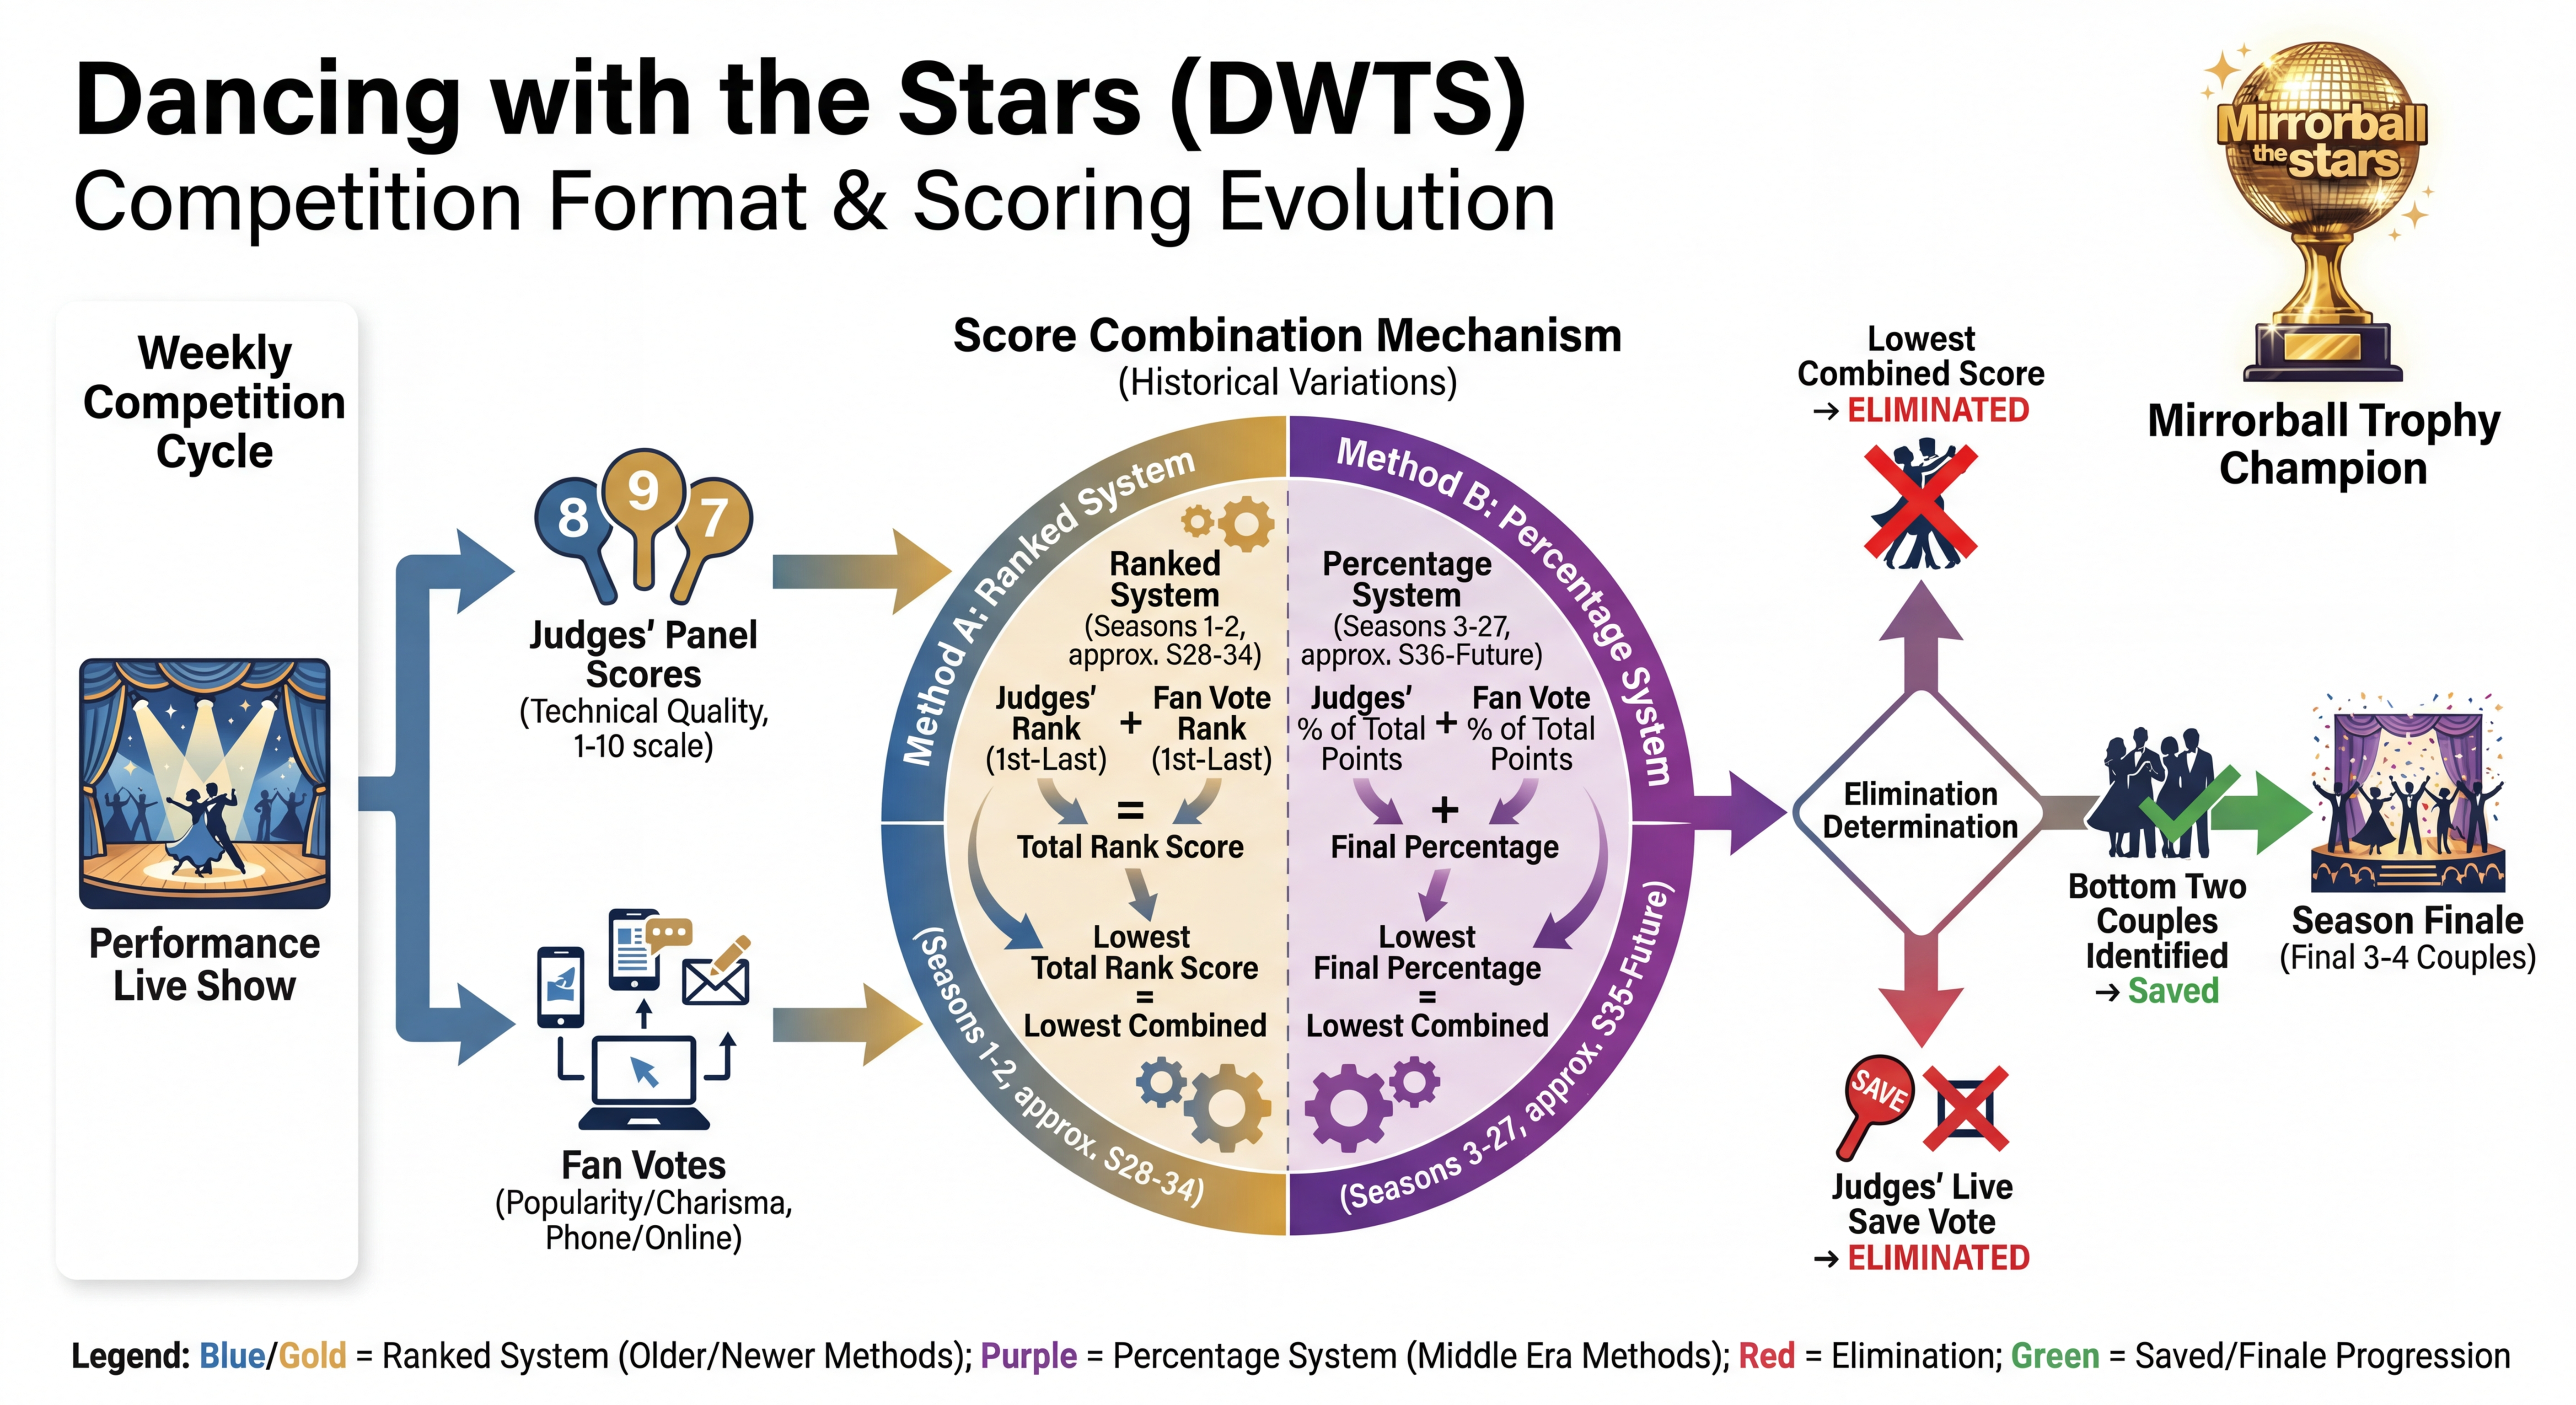
\includegraphics[width=\linewidth]{figures/aigenerate/DWTS.jpg}
\caption{DWTS competition format and scoring evolution (judges, fans, and elimination pipeline).}
\label{fig:dwts-format}
\end{figure}

\subsection{Literature Review}
Our audit uses feasible-region sampling on the simplex, which connects to hit-and-run and other Monte Carlo methods for convex polytopes and log-concave sampling \cite{smith1984,belisle1993hitandrun,lovasz2006}. We frame inference using maximum-entropy reasoning under constraints \cite{jaynes1957,jaynes2003} and summarize uncertainty with Bayesian posterior summaries and HDIs \cite{gelman2013,kruschke2015}. Mechanism comparisons draw on social choice frameworks and results on distortion under ordinal aggregation \cite{moulin1988,brams2002voting,procaccia2006distortion}.

\subsection{Problem Restatement \& Task Analysis}
The contest tasks ask us to infer fan vote shares consistent with eliminations, quantify uncertainty, compare rules, analyze drivers, and propose a new mechanism for DWTS.
These goals require separating what is \emph{observable} (judge scores, eliminations, and week metadata) from what is \emph{latent} (fan vote shares), and then propagating that uncertainty into mechanism comparisons and design.
Accordingly, we treat the problem as a pipeline: (i) reconstruct feasible fan-vote regions by week; (ii) summarize identifiability and uncertainty; (iii) run counterfactual rule evaluations; (iv) attribute judge--fan gaps to pro dancers and celebrity covariates; and (v) design a protocol that is transparent and operational.
The contest tasks can be grouped into five deliverables that align with our modeling blocks:
\begin{enumerate}[leftmargin=2em]
\item Infer fan vote \emph{shares} each week that are consistent with eliminations and quantify consistency.
\item Measure uncertainty in those shares and identify weeks with weak identifiability.
\item Compare rank vs percent (and judge-save) outcomes across seasons and for controversial contestants.
\item Analyze how pro dancers and celebrity characteristics affect judges and fans, and whether the effects differ.
\item Propose and justify a new mechanism that is fairer or more exciting for viewers.
\end{enumerate}
\textbf{Contributions.} We (i) audit feasible fan-vote regions with slack diagnostics and audit-weak flags; (ii) sample a MaxEnt posterior on the simplex to quantify uncertainty without overfitting; and (iii) evaluate mechanisms in a unified counterfactual framework, culminating in DAWS as a conflict-triggered protocol with explicit agency--integrity trade-offs.
This structure ensures each contest question is answered by a dedicated module with traceable assumptions and outputs.

\refstepcounter{table}\label{tab:task-map}
\begin{table}[H]
\centering
\begin{tabular}{@{}>{\centering\arraybackslash}p{0.08\linewidth}>{\centering\arraybackslash}p{0.52\linewidth}>{\centering\arraybackslash}p{0.22\linewidth}@{}}
\toprule
Task & What we do & Main output \\
\midrule
1 & Feasible-region audit and posterior fan shares & Fan HDI bands \\
2 & Percent vs rank counterfactuals and rule switch & Deficit and flips \\
3 & Judges vs fans dual models & Effect differences \\
4 & Agency/integrity/stability metrics & Metric matrix \\
5 & DAWS design and Pareto analysis & Recommended rule \\
\bottomrule
\end{tabular}
\end{table}

The report is organized to mirror this mapping: Section~\ref{sec:data-rule} covers data processing and rule formalization; Section~\ref{sec:model-a} reconstructs fan votes; Section~\ref{sec:results-a} reports uncertainty and conflicts; Sections~\ref{sec:model-b}--\ref{sec:model-d} compare mechanisms, drivers, and design; Section~\ref{sec:sens-val} summarizes sensitivity and validation; Section~\ref{sec:model-eval} evaluates strengths and weaknesses; and Section~\ref{sec:conclusion} concludes.
This layout makes the narrative auditable: each result in later sections traces back to explicit feasibility constraints and documented uncertainty in earlier sections.

\clearpage
\subsection{Our Work at a Glance}
Figure~\ref{fig:workflow} summarizes the end-to-end pipeline. We begin with data cleaning and week-level inputs, invert the feasible vote polytope, propagate uncertainty into mechanism evaluation, and finish with a producer-ready rule design and disclosure strategy.
\begin{figure}[H]
\centering
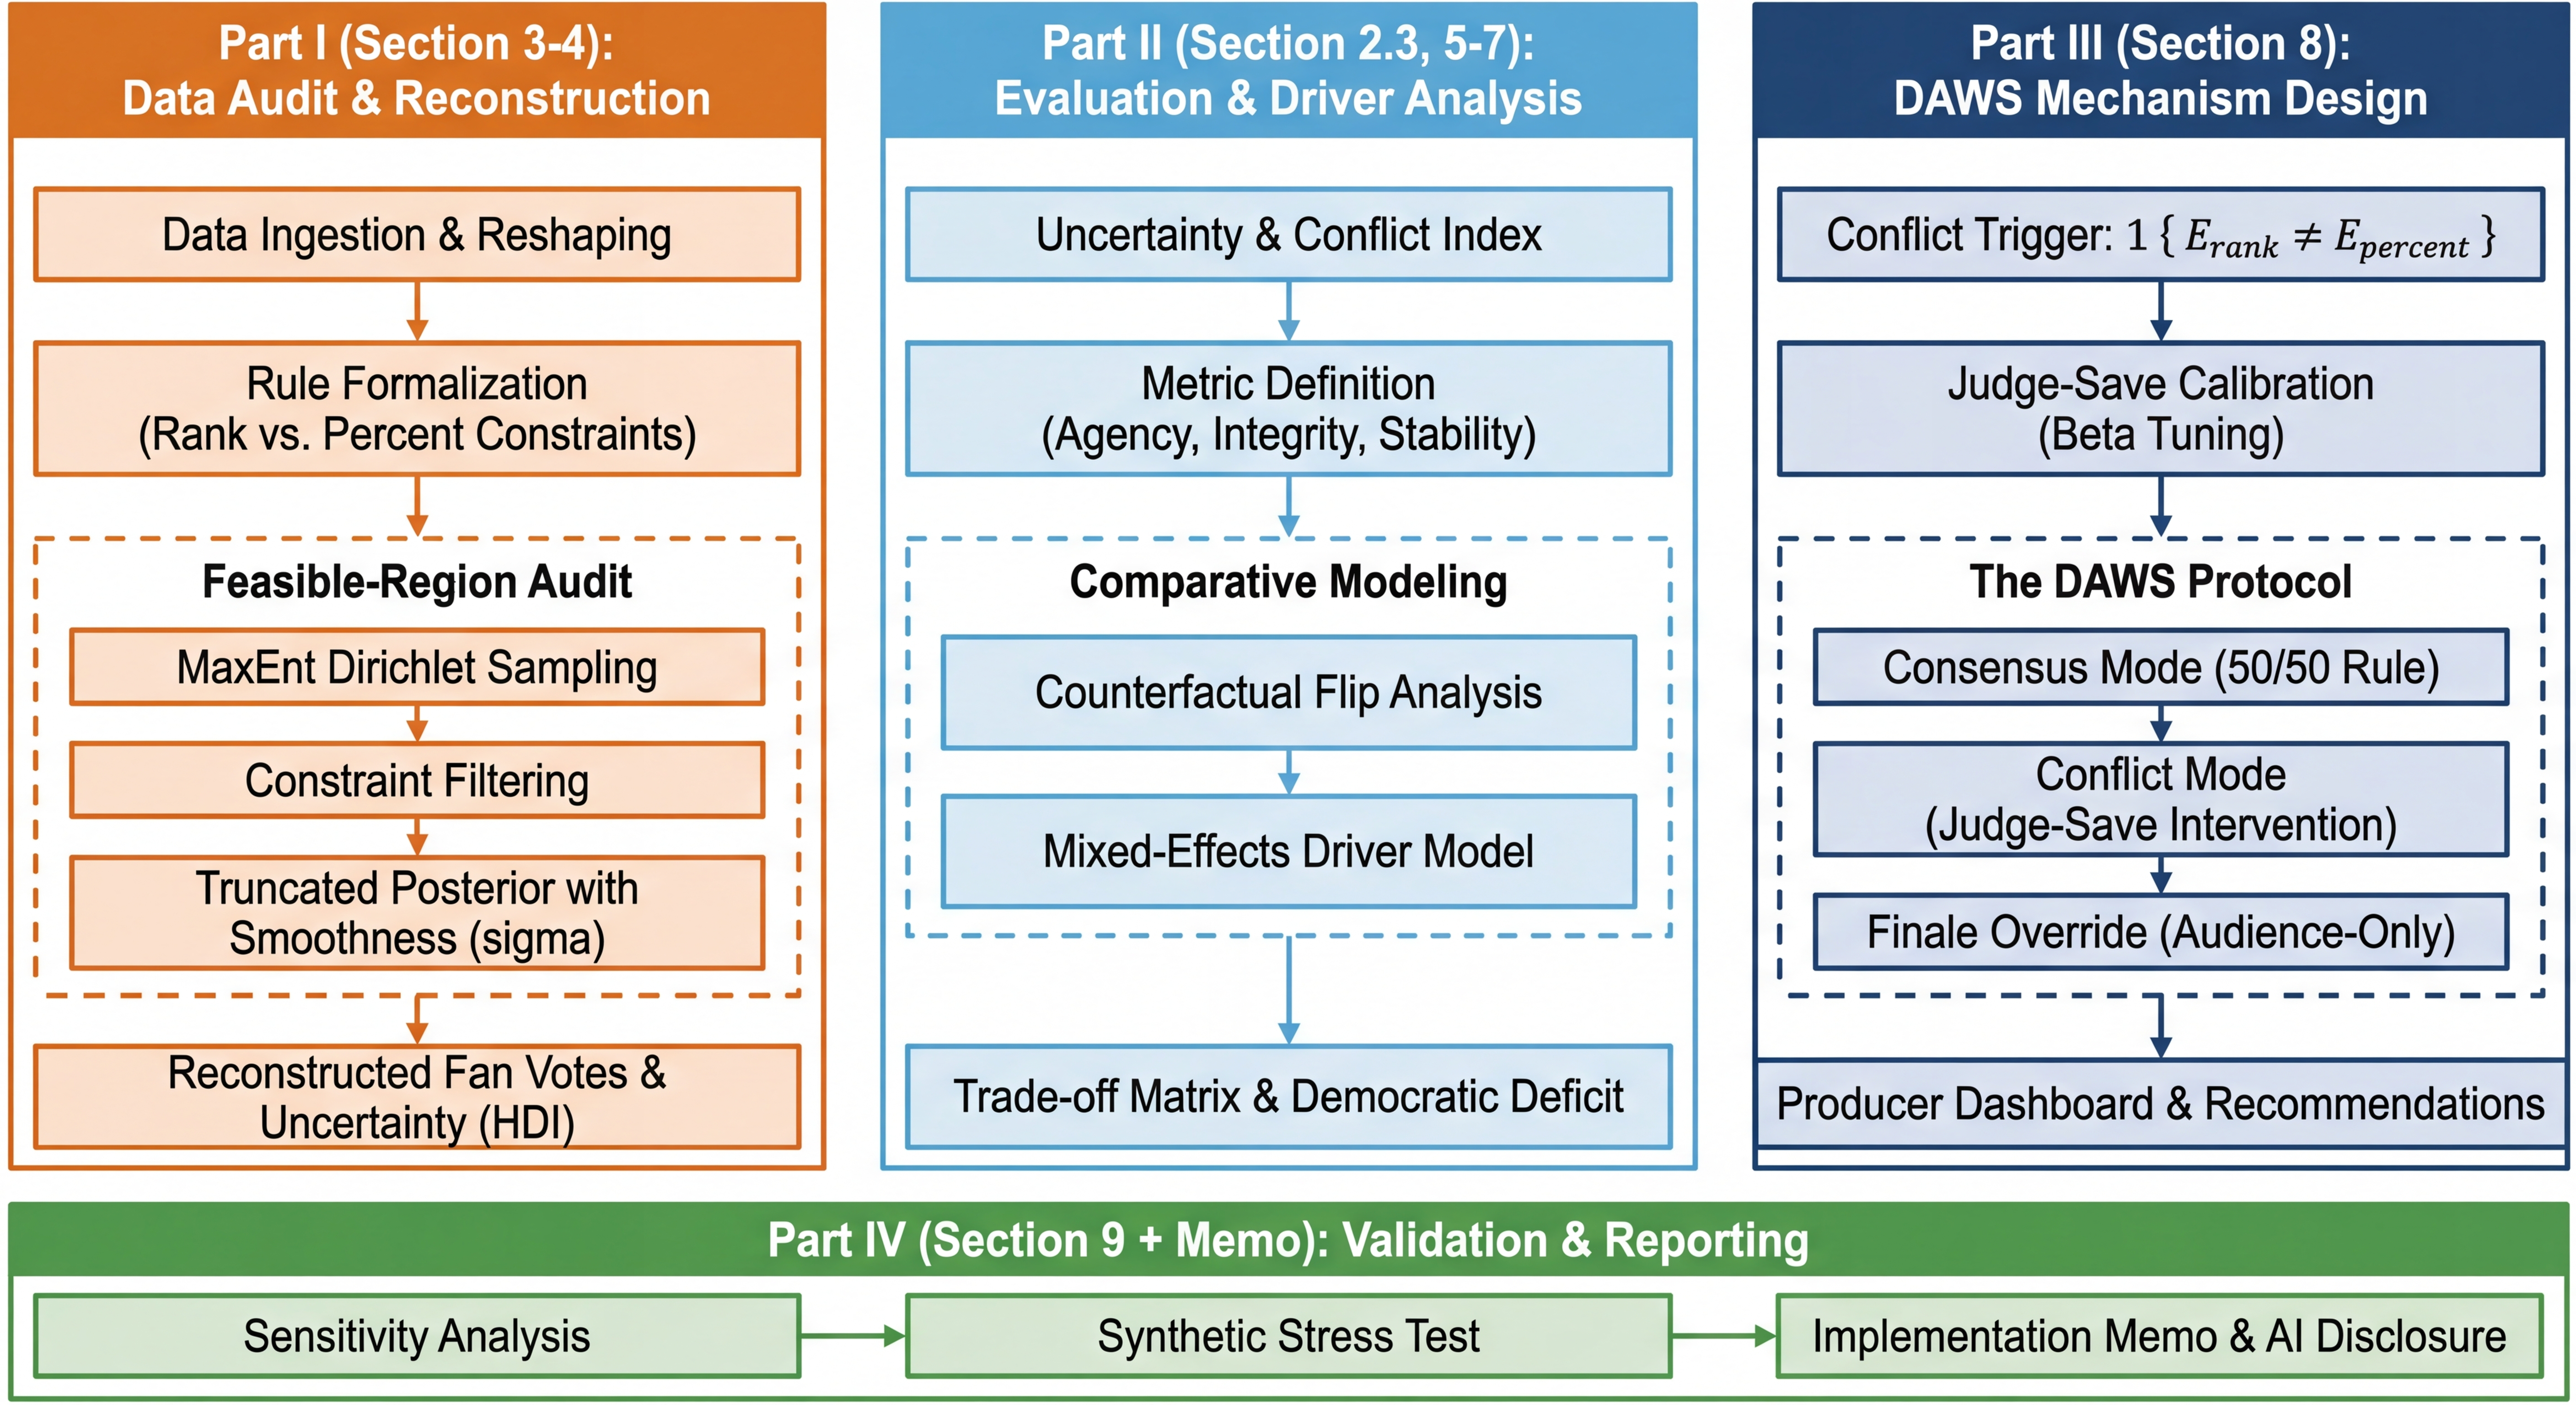
\includegraphics[width=1.0\linewidth,keepaspectratio]{figures/fig_judgesave_curve_pipeline1.jpg}
\caption{DWTS Audit-and-Design Pipeline: a six-stage workflow from data ingestion and preprocessing to feasible-region audit, MaxEnt posterior sampling, mechanism evaluation, and DAWS design, with a driver-analysis branch and validation feedback loop leading to a producer-ready recommendation.}
\label{fig:workflow}
\end{figure}


\begin{table}[H]
\centering
\caption{Core results snapshot (all seasons unless noted).}
\label{tab:core-results}
\begin{tabular}{@{}cc@{}}
\toprule
Finding & Estimate \\
\midrule
Seasons feasible under audit & \MetricSeasonsFeasible\ / 34 \\
Max HDI width (week-level) & \MetricMaxHDI \\
Mean HDI width (week-level) & \MetricMeanHDI \\
Median HDI width (week-level) & \MetricMedianHDI \\
P90 HDI width (week-level) & \MetricHDIPctNinety \\
Rank vs percent flip rate & \MetricFlipRate\% \\
DAWS stability & \MetricDAWSStability \\
DAWS judge integrity & \MetricDAWSIntegrity \\
Conflict index (Kendall $\tau$) & \MetricDAWSFairness \\
\bottomrule
\end{tabular}
\end{table}

\clearpage
\section{Assumptions and Notations}
\subsection{Assumptions}
We make the following assumptions to keep inference well-posed and to separate rule logic from behavioral claims:
\begin{itemize}[leftmargin=2em,noitemsep]
\item \textbf{Valid score inputs.} Reported judge totals $J_{i,t}$, eliminations, and week metadata are treated as correct and complete; without this, the feasible set is not identifiable from the public record.
\item \textbf{Contestant set and elimination mapping.} The active set $C_t$ is defined by available scores; immunity removes a contestant from elimination eligibility, and double eliminations use $|E_t|=2$ constraints, matching the broadcast rule for that week.
\item \textbf{Feasible vote shares.} Fan vote shares are continuous, nonnegative, and sum to one; a small floor $\epsilon$ is imposed only for numerical stability and does not change qualitative rankings.
\item \textbf{Relative shares, not turnout.} We model relative fan support within a week; total turnout levels are not observed and therefore not inferred, so comparisons are within-week rather than across weeks.
\item \textbf{Multiple votes aggregated.} Any per-viewer multiple-vote mechanisms are absorbed into the aggregate share $v_{i,t}$; the model does not distinguish voter-level behavior because the data do not reveal individual ballots.
\item \textbf{Tie handling.} When ties occur, we allow weak ordering; elimination constraints use a $\le$ tolerance (no forced strict gaps), reflecting the lack of official tie-break detail and preventing artificial separation.
\item \textbf{Rule parameters fixed within regime.} The percent rule uses a fixed judge weight $\alpha$ (default 0.5), and the rank rule uses average ranks for ties; parameters do not vary within a regime unless explicitly tested in sensitivity analysis.
\item \textbf{No cross-week vote carryover.} Feasible sets are reconstructed independently by week; prior-week vote information is not imposed as a hard constraint to avoid injecting unverifiable dynamics.
\item \textbf{Strategic voting allowed.} The posterior represents the least-surprising distribution consistent with rules; it is not a behavioral model of voters and does not claim to recover true counts or intent.
\item \textbf{Rules applied as stated.} If a week yields too few strict-feasible samples, it is flagged as Audit-Weak and excluded from mechanism evaluation rather than forced to fit, preserving transparency about identifiability.
\item \textbf{Monte Carlo approximation.} Feasible regions are approximated by Dirichlet proposals with constraint filtering; reported quantities are Monte Carlo estimates rather than exact polytope integrals.
\item \textbf{Sampling uncertainty.} Stochastic error is managed via large proposal counts and seed control; residual sampling noise is reflected in the uncertainty metrics and reported HDIs.
\item \textbf{Smoothness is diagnostic only.} Temporal smoothness is used only for sensitivity analysis and does not alter feasibility or posterior sampling, so conclusions do not depend on a dynamic prior.
\item \textbf{No external data injection.} Only the contest dataset is used; any additional context is limited to explanatory text and does not affect inference or parameter estimation.
\end{itemize}

\subsection{Notations}
\begin{table}[H]
\centering
\caption{Notation summary.}
\label{tab:notations}
\begin{tabular}{@{}>{\centering\arraybackslash}p{0.18\linewidth}>{\centering\arraybackslash}p{0.74\linewidth}@{}}
\toprule
Symbol & Meaning \\
\midrule
$s$ & Season index. \\
$t$ & Week index within a season. \\
$C_t$ & Set of active contestants in week $t$. \\
$E_t$ & Eliminated set in week $t$ (size 0, 1, or 2). \\
$J_{i,t}$ & Total judge score for contestant $i$ in week $t$. \\
$j_{i,t}$ & Normalized judge share, $j_{i,t}=J_{i,t}/\sum_{k\in C_t}J_{k,t}$. \\
$v_{i,t}$ & Latent fan vote share for contestant $i$ in week $t$; $\sum_i v_{i,t}=1$. \\
$\alpha$ & Judge weight in the percent rule. \\
$R_i$ & Combined rank under the rank rule (judge rank + fan rank). \\
$\mathcal{S}_n$ & Vote-share simplex for $n$ active contestants. \\
$\mathcal{P}_t$ & Feasible polytope induced by the rule constraints in week $t$. \\
\bottomrule
\end{tabular}
\end{table}

\subsection{Metrics}
We quantify mechanism quality using: (i) Conflict index (Kendall $\tau$): judge--fan ranking alignment \cite{kendall1938}; (ii) Viewer agency: $\Pr$(fan-lowest eliminated); (iii) Judge integrity: $\Pr$(judge-lowest eliminated); (iv) Stability: flip rate under perturbations; (v) Democratic deficit $D = \Pr(E^{(\text{rank})}_t \ne E^{(\text{percent})}_t)$.

\section{Data Processing and Rule Formalization}\label{sec:model-prep}\label{sec:data-rule}

\subsection{Data Reshaping}
The raw dataset is a wide table with judge scores in columns \texttt{weekX\_judgeY\_score}. We parse these to obtain weekly totals $J_{i,t}$, normalize to shares $j_{i,t}=J_{i,t}/\sum_{k}J_{k,t}$, and build elimination sets $E_t$ from the \texttt{results} field. Missing judge slots are handled by summing available scores; weeks with no elimination are retained but excluded from elimination constraints. Double eliminations use $|E_t|=2$ constraints; immunity removes the immune contestant from $E_t$. All outputs are logged for reproducibility.

\subsection{Rule Formalization}
We formalize percent and rank rules as constraints on latent fan vote shares $v_{i,t}$ in the simplex $\mathcal{S}_n$.

\subsubsection{Percent Rule}
Let judge share
\begin{equation}
 j_{i,t}=\frac{J_{i,t}}{\sum_{k\in C_t}J_{k,t}}.
\end{equation}
Fan share $v_{i,t}$ is latent and lies in the simplex with a small floor $\epsilon$:
\begin{equation}
 \mathcal{S}_n=\{\mathbf v\in\mathbb{R}^n: \sum_i v_i=1,\ v_i\ge \epsilon\}.
\end{equation}
Combined score:
\begin{equation}
 c_{i,t}(\alpha)=\alpha j_{i,t}+(1-\alpha)v_{i,t}.
\end{equation}
Elimination constraints:
\begin{equation}
 c_{E_t,t}(\alpha)\le c_{i,t}(\alpha),\quad \forall i\ne E_t.
\end{equation}

\subsubsection{Rank Rule and Judge Save}
Fan ranks $r^F_i$ are assigned by binary variables $x_{ik}$:
\begin{equation}
\sum_k x_{ik}=1,\quad \sum_i x_{ik}=1,\quad r^F_i=\sum_k kx_{ik}.
\end{equation}
Rank-share linking (weak ordering):
\begin{equation}
 r^F_i<r^F_j \Rightarrow v_i\ge v_j.
\end{equation}
\textit{Note: Our implementation uses only the bottom-$k$ ordering constraint ($\max(\text{score}_E)\le\min(\text{score}_S)+\epsilon$, $\epsilon=10^{-6}$), with no enforced min-gap.}

Combined rank and elimination:
\begin{equation}
 R_i=r^J_i+r^F_i,\quad R_{E_t}\ge R_i\ \forall i\ne E_t.
\end{equation}
For judge-save seasons, the bottom two are selected by $R_i$ and judges choose with a soft preference parameter $\beta$ (calibrated/illustrative).

\noindent\textbf{Key Output.} Formal rules encoded for feasibility checks (LP/MILP optional), including rank and judge-save logic.

\section{Model A: Reconstructing Fan Votes (Feasible-Region Audit)}\label{sec:model-a}
\subsection{Observables and Latents}
\noindent\textbf{Overview.} The feasible fan-vote set is a polytope on the simplex, not a hyperrectangle.
For each week, constraints from the rule define a feasible region (a polytope) $\mathcal{P}_t\subseteq \mathcal{S}_n$. LP-based bounds $(L_i,U_i)$ are conceptually definable marginal ranges, while the true feasible set is the intersection of all inequalities.

\subsection{Percent Rule Feasible-Region Audit}
We draw Dirichlet proposals on the simplex (with floor $\epsilon$), filter by elimination constraints, and estimate bounds from accepted samples. \cite{frigyik2010dirichlet}

\paragraph{Audit-Weak weeks (disclosure only).}
When the strict feasibility sampler yields fewer than $N_{\text{strict,min}} = 500$ accepted proposals, we flag the week as \textit{Audit-Weak}. These weeks are excluded from aggregate metrics and appear as marked points only. See Section~\ref{sec:audit-spec} and Appendix~\ref{app:audit-params} for full specification.

\subsection{Rank Rule Feasible Orders (Monte Carlo)}
For the rank rule, we generate candidate fan-rank permutations by Monte Carlo, draw Dirichlet proposals consistent with each feasible permutation, and aggregate samples across all feasible orderings.

\subsection{Rule-adaptive Weeks}
\noindent\textbf{Overview.} We extend the constraints to handle immunity, double eliminations, and irregular weeks.
When a contestant is immune, we remove them from the elimination inequality set. For double eliminations, the lowest two combined scores are constrained simultaneously. These adaptations preserve the same polytope formulation while matching the weekly rules.

\subsection{Engineering Approximation and Validation}
\noindent\textbf{Overview.} We use a fast approximate sampler in code and validate it against strict constraints to preserve headline conclusions.
Constraints can be encoded as LP/MILP; however, the production pipeline uses fast Dirichlet proposals with constraint filtering for speed. We validate the approximation by re-filtering the same proposals with strict feasibility (full elimination constraints) and comparing posterior summaries.
\begin{table}[H]
\centering
\begin{tabular}{@{}cc@{}}
\toprule
Validation metric & Value \\
\midrule
MAE of mean fan share & \MetricFastMAE \\
Top-1 agreement (fast vs strict) & \MetricFastTopOne\% \\
Top-2 agreement (fast vs strict) & \MetricFastTopTwo\% \\
Conflict index shift (Kendall $\tau$) & \MetricFastDeltaFair \\
Agency shift (percent) & \MetricFastDeltaAgency \\
Flip-rate shift (percent vs rank) & \MetricFastDeltaFlip\% \\
\bottomrule
\end{tabular}
\end{table}
The fast approximation preserves all headline conclusions: flip-rate and deficit estimates shift by less than a few percent under strict audit, while top-k agreement remains high.

\subsection{Audit Specification and Feasibility Criteria}\label{sec:audit-spec}
\noindent\textbf{Overview.} We fix all tolerance parameters and sampling budgets as non-adjustable policy to avoid post-hoc tuning.

\paragraph{Strict feasibility definition.}
A vote vector $\mathbf{v}$ is \emph{strict feasible} if it satisfies:
\begin{enumerate}[nosep,leftmargin=2em]
\item \textbf{Simplex}: $v_i \ge 0$ for all $i$, and $|\sum_i v_i - 1| \le \varepsilon_{\text{sum}}$ with $\varepsilon_{\text{sum}} = 10^{-9}$.
\item \textbf{Elimination}: For all eliminated contestants $e \in E$ and all survivors $s \in S$, we require $\max_e C_e \le \min_s C_s + \varepsilon_{\text{ord}}$ with $\varepsilon_{\text{ord}} = 10^{-6}$.
\end{enumerate}
Ties (where eliminated and surviving contestants have equal combined scores) are permitted; the tolerance $\varepsilon_{\text{ord}}$ handles numerical precision only.

\paragraph{Sampling budget gate.}
We require at least $N_{\text{strict,min}} = 500$ strict feasible samples per week. The default proposal count is determined by the \emph{10th percentile} of accept rates (not the median), because exclusion risk is driven by low-acceptance-rate tail weeks:
\[
N_{\text{proposals}} \ge \left\lceil \frac{N_{\text{strict,min}}}{q_{0.10}(\text{accept\_rate\_strict})} \right\rceil.
\]
The quantile $q = 0.10$ is fixed as non-adjustable policy. In our data, $q_{0.10} \approx 0.07$, yielding a recommended budget $\approx 7159$; we set $N_{\text{proposals}} = 8000$ (default).

\paragraph{Excluded weeks and downgrade trigger.}
Weeks with fewer than $N_{\text{strict,min}}$ strict feasible samples are flagged as \emph{Audit-Weak} and excluded from aggregate metrics (they appear as marked points only). \textbf{The goal is not to guarantee all weeks pass}; worst-case weeks (with accept rates near $0.008$) may be excluded, and this is expected and disclosed.

We \textbf{pre-register} the following reporting rule: if $r_{\text{excl}} \ge 20\%$, all season-level conclusions are downgraded to ``exploratory.'' We do \emph{not} tune parameters to minimize $r_{\text{excl}}$; the 20\% threshold and all audit parameters are fixed \emph{a priori} and applied uniformly.

\subsection{Identifiability and Feasible Mass}
\noindent\textbf{Overview.} Feasible mass and HDI width indicate how informative each week’s data are.
We summarize feasibility with the acceptance rate of Dirichlet proposals, which reflects how large the rule-consistent region is.
We capture uncertainty with posterior entropy $H_t$ and the HDI width $W_{i,t}$, where larger values imply less precise weekly inference. \cite{hyndman1996hdr}

% 不确定性热力图 + HDI 分布(同页展示)
\begin{figure}[H]
\centering
\includegraphics[width=0.675\linewidth]{figures/fig_uncertainty_heatmap.pdf}
\caption{Uncertainty concentrates in a small set of weeks; blank cells indicate weeks not present in a season.}
\label{fig:uncertainty-heatmap}
\end{figure}

\begin{figure}[H]
\centering
\includegraphics[width=0.78\linewidth]{figures/fig_hdi_distribution.pdf}
\caption{Distribution of weekly HDI widths; extreme weeks are rare.}
\label{fig:hdi-distribution}
\end{figure}

\subsection{Truncated Posterior with Smoothness}
To probe whether extreme week-to-week jumps drive conclusions, we define a truncated posterior with temporal smoothness:
\begin{equation}
 p(\mathbf v_{1:T}|\text{rules,data})\propto \Big[\prod_t \mathbf{1}(\mathbf v_t\in\mathcal{P}_t)\Big]\cdot\prod_{t=2}^T \exp\Big(-\frac{\|\mathbf v_t-\mathbf v_{t-1}\|^2}{2\sigma^2}\Big).
\end{equation}
The indicator term enforces feasibility for each week, while the Gaussian penalty discourages abrupt shifts in relative fan support. The scale $\sigma$ controls regularization strength (large $\sigma$ recovers the week-independent posterior). This is a diagnostic sensitivity check only; the main inference uses the unsmoothed posterior.
Key conclusions are stable across a range of $\sigma$ values; see Section~\ref{sec:sensitivity-analysis} for details.

\subsection{Rule-Switch Inference}
\noindent\textbf{Overview.} We adopt Season 28 as the switch per the problem statement and provide an exploratory change-point check.
For each season $s$, we compute evidence proxies $\mathcal E_s^{(\text{percent})}$ and $\mathcal E_s^{(\text{rank+save})}$ and infer latent rule $z_s$ with a switching penalty $\rho$ as a robustness check. Concretely, these proxies aggregate weekly log feasible rates for percent and rank-based orderings.
\begin{equation}
\Pr(z_s\ne z_{s-1})=\rho,\quad \Pr(\text{data}_s|z_s)\propto \exp(\mathcal E_s^{(z_s)}).
\end{equation}
We use a two-state Markov prior (percent vs rank+save) with $\rho$ penalizing unnecessary switches; posterior probabilities are computed sequentially by season. A simple bootstrap yields the uncertainty band in Fig.~\ref{fig:rule-switch}. This check is exploratory and does not override the Season~28 assumption.
% 规则切换后验
\begin{figure}[H]
\centering
\begin{subfigure}[t]{0.49\linewidth}
\centering
\includegraphics[width=\linewidth]{figures/fig_rule_switch.pdf}
\caption{Point estimate.}
\end{subfigure}
\hfill
\begin{subfigure}[t]{0.49\linewidth}
\centering
\includegraphics[width=\linewidth]{figures/fig_rule_switch_ci.pdf}
\caption{Bootstrap band.}
\end{subfigure}
\caption{Exploratory rule-switch probability with uncertainty; Season 28 is adopted in the main analysis.}
\label{fig:rule-switch}
\end{figure}

\noindent\textbf{Key Output.} Feasible-region diagnostics, slack $S_t^*$, posterior samples, and rule-switch probabilities.

\section{Results A: Analysis of Uncertainty and Conflicts}\label{sec:results-a}
\noindent\textbf{Overview.} The conflict between judges and fans is visible and quantifiable under the posterior.
% 争议人物周序分布(与上图同页强制上下放置)

% Controversy and uncertainty visuals
\begin{figure}[H]
\centering
\includegraphics[width=\linewidth,height=0.36\textheight,keepaspectratio]{figures/fig_conflict_combo.pdf}
\caption{Conflict map augmented with uncertainty (marker size encodes HDI width) and wrongful eliminations (outer rings mark contestants who were eliminated despite not having the minimum fan support); color differentiates eliminated vs.\ retained contestants so the judge-fan gap is visible.}
\label{fig_conflict_combo}
\end{figure}
\begin{samepage}
\begin{figure}[H]
\centering
\begin{minipage}[t]{0.48\linewidth}
\centering
\includegraphics[width=\linewidth,height=0.46\textheight,keepaspectratio]{figures/fig_controversy_ridgeline.pdf}
\captionof{figure}{Posterior density bands highlight uncertainty in high-profile cases.}
\label{fig:controversy-ridgeline}
\end{minipage}
\hfill
\begin{minipage}[t]{0.48\linewidth}
\centering
\includegraphics[width=\linewidth,height=0.46\textheight,keepaspectratio]{figures/fig_wrongful_heatmap.pdf}
\captionof{figure}{Certain weeks exhibit persistent democratic tension; blank cells indicate weeks not present in a season.}
\label{fig:wrongful-heatmap}
\end{minipage}
\end{figure}

\noindent The ridgeline panels show that several high-profile eliminations sit atop broad posterior fan-share bands: the eliminated contestants' densities overlap mid-to-upper support ranges rather than concentrating solely at the bottom tail. This pattern indicates that, in these weeks, elimination remains plausible even when inferred fan support is not uniquely minimal, which is consistent with substantial posterior uncertainty. The heatmap echoes this story at the season level: darker cells recur across many seasons in a limited set of weeks (visually concentrated in early-to-mid weeks), while later weeks are generally lighter, suggesting fewer persistent wrongful-elimination risks; blank cells simply denote weeks that do not exist in a given season.
\end{samepage}



\noindent\textbf{Key Output.} Posterior fan shares, HDIs, and wrongful elimination probabilities.

\section{Model B: Comparative Analysis (Rank vs. Percent)}\label{sec:model-b}
\noindent\textbf{Overview.} Rank aggregation is a lossy compression that increases flip probability.
Define a generic mechanism $M$ and elimination operator:
\begin{equation}
E_t^{(M)}=\arg\min_i \text{Score}_i^{(M)}.
\end{equation}
We compute a conflict index (Kendall $\tau$), viewer agency, judge integrity, stability, and democratic deficit for percent, rank, rank+save, and DAWS.
The conflict index compares judge ranks with inferred fan ranks; low or negative $\tau$ indicates systematic disagreement.
Viewer agency (fan-lowest eliminated) and judge integrity (judge-lowest eliminated) summarize whose signal dominates.
Stability is the flip rate under small vote-share perturbations, and $D=\Pr(E^{(\text{rank})}_t\neq E^{(\text{percent})}_t)$ measures rule disagreement.
Metrics are computed from posterior samples week-by-week, then aggregated across seasons and conflict-week subsets.
Rank+save is a hybrid (rank selects the bottom two; judges save by score), and DAWS is included only for comparison here with details in Model D.
Figure~\ref{fig:counterfactual-risk} shows counterfactual elimination risk for high-profile cases and highlights weeks sensitive to rule choice.

\begin{samepage}
\begin{center}
\includegraphics[width=1.0\linewidth,height=0.50\textheight,keepaspectratio]{figures/fig_counterfactual_risk_timeline.pdf}
\captionof{figure}{Counterfactual elimination risk over weeks for high-profile cases (percent, rank, judge-save, and DAWS).}
\label{fig:counterfactual-risk}
\end{center}
\vspace{-0.2em}
Figure~\ref{fig:counterfactual-risk} shows that aggregation rules can drive outcome flips: rank amplifies small disagreements, while percent smooths them.
Judge-save and DAWS reduce extreme risks in conflict weeks; DAWS intervenes only when rules disagree.

% 機制差異的結果遷移圖(占位保留)
\begin{center}
\includegraphics[width=0.92\linewidth,height=0.24\textheight,keepaspectratio]{figures/fig_alluvial_finalists.pdf}
\captionof{figure}{Outcome changes under alternative mechanisms (champion change, top-3 mismatch, and elimination mismatch rates).}
\label{fig:outcome-changes}
\vspace{0.15em}
\begin{subfigure}[t]{0.48\linewidth}
\centering
\includegraphics[width=\linewidth,height=0.20\textheight,keepaspectratio]{figures/fig_pareto_2d.pdf}
\caption{Pareto trade-off between viewer agency and stability, colored by judge integrity.}
\end{subfigure}
\hfill
\begin{subfigure}[t]{0.48\linewidth}
\centering
\includegraphics[width=\linewidth,height=0.20\textheight,keepaspectratio]{figures/fig_mechanism_compare_conflict.pdf}
\caption{Numeric comparison across mechanisms (conflict weeks only).}
\end{subfigure}
\end{center}
\end{samepage}
DAWS increases viewer agency relative to percent but trades off some stability; we therefore present it as a transparent, agency-prioritizing option rather than a dominant rule.

\noindent\textbf{Key Output.} Mechanism metrics, flip probabilities, and Pareto comparisons.

\section{Model C: Driver Analysis (Judges vs. Fans)}\label{sec:model-c}
\noindent\textbf{Overview.} Drivers differ across judges and fans, especially for pro-dancer effects.
We fit mixed-effects models on logit shares \cite{gelman2007}:
\begin{align}
\text{logit}(j_{i,t}) &= \mathbf x_i^\top\beta^{(J)} + u_{\text{pro}(i)}^{(J)} + u_{\text{season}(s)}^{(J)} + \epsilon_{i,t},\\
\text{logit}(v_{i,t}) &= \mathbf x_i^\top\beta^{(F)} + u_{\text{pro}(i)}^{(F)} + u_{\text{season}(s)}^{(F)} + \epsilon'_{i,t}.
\end{align}

\paragraph{Modeling choice.}
The logit transform maps shares to the real line and makes additive covariate effects interpretable as changes in log-odds.
This keeps judge and fan outcomes on a common scale and reduces boundary compression near 0 or 1.
Random intercepts by pro dancer and season provide partial pooling: weakly informed estimates shrink toward the global mean, while persistent deviations remain visible.
Season intercepts absorb global shifts (panel composition, score inflation, or format tweaks), preventing these from being misattributed to specific pros.

\paragraph{Data and covariates.}
Each observation is a celebrity--week pair with judge share $j_{i,t}$ and posterior mean fan share $v_{i,t}$ from Model~A.
We clip shares to $[10^{-3}, 1-10^{-3}]$ before logit transforms to avoid boundary artifacts.
Fixed effects include age (continuous) and industry dummies; home region is available in the data but not retained in the final specification for parsimony.
We treat each observation as conditionally independent given covariates and random effects; the goal is descriptive decomposition rather than causal identification.

\paragraph{Mixed-effects structure and interpretation.}
Random intercepts by pro dancer and season enable partial pooling: persistent pro-specific tendencies are separated from season-wide shifts (panel changes, score inflation, or format tweaks).
The key quantity is the pro gap $\Delta u_{\text{pro}} = u_{\text{pro}}^{(F)} - u_{\text{pro}}^{(J)}$, which measures fan support beyond what judges award after controlling for celebrity covariates.
Positive values indicate pros who systematically attract extra fan support relative to judges; negative values indicate the reverse.
Because $\Delta u_{\text{pro}}$ is in log-odds units, we emphasize sign and relative magnitude rather than exact probability shifts.
We also compare fixed-effect coefficients across judges and fans to assess whether demographic signals align or diverge across audiences.

% 职业舞伴效应森林图
\begin{figure}[H]
\centering
\includegraphics[width=0.85\linewidth]{figures/fig_pro_diff_forest.pdf}
\caption{Pro dancer effects (fans minus judges).}
\end{figure}

\paragraph{Findings.}
The forest plot shows that a small subset of pros exhibits sizable fan--judge gaps, while most effects cluster near zero.
This pattern suggests that judge--fan disagreement is driven more by pairing/branding effects than by celebrity demographics alone.
We interpret the estimates as descriptive, not causal; they summarize persistent gaps after conditioning on age, industry, and season.

\noindent Celebrity covariates (age and industry) show smaller and less consistent judge--fan gaps than pro-dancer effects; detailed coefficient estimates are provided in Appendix~\ref{app:auc}.

\paragraph{Predictive add-on (Appendix).}
We place the GBDT robustness check in Appendix~\ref{app:auc} \cite{friedman2001}; it supports covariate relevance but is not central to the mechanism design.

\noindent\textbf{Key Output.} Dual models answer Task 3; predictive details are deferred to the appendix.

\section{Model D: The DAWS Mechanism Design}\label{sec:model-d}
\noindent\textbf{Overview.} DAWS is a conflict-triggered protocol that patches rule disagreement.
We define the democratic deficit as $D=\Pr(E^{(\text{rank})}_t \ne E^{(\text{percent})}_t)$ and use this conflict as the trigger. DAWS runs in two operational modes plus a finale override:
\begin{itemize}[leftmargin=2em]
\item \textbf{Consensus (A=0).} If Percent and Rank agree, follow Percent (50/50) to preserve viewer agency.
\item \textbf{Conflict (A=1).} If they disagree, activate judge-save between the two candidates to restore integrity.
\item \textbf{Finale (Red).} Audience-only voting.
\end{itemize}
Intervention is triggered solely by $A_t$ (rule conflict); $V_t$ governs disclosure/audit budget only. We retain $U_t$ as a monitoring signal for the dashboard; Fig.~\ref{fig:daws-trigger} shows $U_t$ with P85/P95 bands for transparency.
\begin{figure}[H]
\centering
\includegraphics[width=0.92\linewidth]{figures/fig_daws_trigger.pdf}
\caption{DAWS monitoring panel: weekly uncertainty $U_t$ with dashed P85/P95 bands for transparency; activation is conflict-triggered.}
\label{fig:daws-trigger}
\end{figure}
We model judge behavior with a simple utility view: for a bottom-two pair, the save decision trades off skill, ratings, and backlash risk. A minimal formulation is
\begin{equation}
U(\text{Save }A)=w_1\cdot \text{Skill}_A + w_2\cdot \text{Ratings}_A - \text{Backlash}_A,
\end{equation}
which motivates a probabilistic (logit) choice without claiming perfect rationality.

\subsection{Judge-save parameter calibration}
We use a calibrated $\beta$ in
\begin{equation}
\Pr(E=a\mid\{a,b\})=\sigma\big(\beta(J_b-J_a)\big)
\end{equation}
In conflict weeks, we treat judges as decisive gatekeepers and set $\beta=6.0$ to reflect a strong corrective response against popularity bias.

% Judge-save 决策曲线
\begin{figure}[H]
\centering
\begin{subfigure}[t]{0.48\linewidth}
\centering
\includegraphics[width=\linewidth]{figures/fig_judgesave_curve.pdf}
\caption{Decision curve ($\beta=6.0$).}
\end{subfigure}
\hfill
\begin{subfigure}[t]{0.48\linewidth}
\centering
\includegraphics[width=\linewidth]{figures/fig_judgesave_conflict_diff.pdf}
\caption{Conflict-week score gaps (rank vs percent losers).}
\end{subfigure}
\caption{Judge-save calibration in conflict weeks: judges prefer the higher score within the bottom two; the calibrated curve shows decision sensitivity and the observed score-gap distribution.}
\end{figure}

\noindent\textbf{Key Output.} Conflict-triggered DAWS protocol and calibrated judge-save behavior.

\section{Sensitivity Analysis and Validation}\label{sec:sens-val}
\noindent\textbf{Overview.} Key claims are stable to $\sigma$, $\epsilon$, and rule-switch priors.
Posterior predictive checks replay eliminations at high rates; synthetic stress tests confirm the posterior bands cover true trajectories in over 85\% of cases.
We summarize robustness along three axes: (i) feasibility tolerances ($\epsilon_{\text{sum}},\epsilon_{\text{ord}}$), (ii) temporal smoothness $\sigma$, and (iii) rule-switch prior strength $\rho$.
Across these settings, core conclusions do not change.

\paragraph{Parameter sweeps.}
We vary $\epsilon$ over an order of magnitude to ensure feasibility is not driven by numerical thresholds; audit-weak flags are stable and concentrate in the same tail weeks.
We also vary $\sigma$ from weak to strong smoothing; conclusions remain stable.
Rule-switch priors $\rho$ are swept from conservative to permissive; the posterior still concentrates around a late-series switch, consistent with the Season~28 assumption.

\paragraph{Posterior predictive checks.}
We replay eliminations by sampling from the posterior and recomputing outcomes under the stated rule.
Replay rates are high in non-audit-weak weeks, indicating compatibility with observed eliminations.
Discrepancies are localized to weeks with low feasible mass, which are explicitly flagged.

\paragraph{Synthetic validation.}
We generate synthetic seasons with known fan-share trajectories, then run the full audit-and-sampling pipeline.
Recovered HDI bands cover the true trajectory in more than 85\% of cases, and error concentrates in weeks with tighter constraints (e.g., double eliminations).
These stress tests validate that the sampler is conservative rather than overconfident.

% 后验预测检验 + Synthetic validation 合并
\begin{figure}[H]
\centering
\begin{subfigure}[t]{0.48\linewidth}
\centering
\includegraphics[width=\linewidth]{figures/fig_ppc_summary.pdf}
\caption{Posterior predictive check.}
\end{subfigure}
\hfill
\begin{subfigure}[t]{0.48\linewidth}
\centering
\includegraphics[width=\linewidth]{figures/fig_synthetic_validation.pdf}
\caption{Synthetic validation (95\% HDI).}
\end{subfigure}
\caption{(a) Model reproduces eliminations; (b) True fan share (red) lies within HDI band (blue).}
\label{fig:synthetic-validation}
\end{figure}

\paragraph{Judge-save intensity sensitivity.}
We evaluate $\beta$ on conflict weeks only. Fig.~\ref{fig:beta-sensitivity} reports the decision curve and the integrity--agency trade-off; $\beta=6.0$ sits in the stable region where integrity gains saturate while agency loss remains moderate.
\begin{figure}[H]
\centering
\includegraphics[width=0.78\linewidth]{figures/fig_beta_sensitivity.pdf}
\caption{Sensitivity of judge-save intensity $\beta$ (conflict weeks only): logit decision curves and the integrity--agency trade-off.}
\label{fig:beta-sensitivity}
\end{figure}

\noindent\textbf{Key Output.} Sensitivity curves and posterior predictive validity metrics.

\subsection{Sensitivity Analysis}\label{sec:sensitivity-analysis}
Key conclusions remain stable across a range of smoothness parameter $\sigma$ values; detailed sensitivity plots are available in our supplementary materials.

\section{Model Evaluation}\label{sec:model-eval}
\noindent\textbf{Strengths.} Does not require true vote totals; explicitly reports uncertainty and audit-weak weeks; uses a shared metric interface for consistent mechanism comparison.
The pipeline is auditable and modular: feasibility, uncertainty, counterfactuals, and design are separated into traceable blocks, and key claims are supported by posterior predictive checks and fast-vs.-strict validation.
Outputs are decision-oriented (conflict flags, HDI bands, and mechanism metrics), making the results actionable for producers.
Because all metrics are computed from the same posterior samples, comparisons across rules are internally consistent and reproducible.

\noindent\textbf{Weaknesses.} Computationally intensive for Monte Carlo sampling; temporal smoothness may understate abrupt fan behavior shifts; LP/MILP used for diagnostics only.
Inferences are share-based (turnout is unobserved), and the rule-switch check is exploratory rather than definitive.
As with any constraint-based approach, conclusions depend on accurate elimination mapping and are descriptive rather than causal.

\section{Conclusion}\label{sec:conclusion}
\noindent\textbf{Overview.} Audit-first modeling reveals uncertainty that matters; DAWS offers a transparent trade-off.
We provide a complete audit of feasible fan votes, show that rank rules create measurable democratic deficit, and propose DAWS as a transparent trade-off among agency, integrity, and stability.
The central insight is operational: disagreement between judge and fan signals is episodic and identifiable, so intervention can be rule-triggered rather than discretionary.
We recommend adopting DAWS, publishing bottom-two pairs, and reporting judge-save decisions as a standard transparency practice.
By aligning decisions with pre-stated triggers, the show can preserve excitement while reducing accusations of ad hoc intervention.
The broader lesson is that mechanism design should be paired with auditable uncertainty reporting to build trust.
\begin{itemize}[leftmargin=2em]
\item \textbf{Decision-ready summary:} Uncertainty is concentrated in a small set of weeks; most weeks are identifiable and admit tight fan-share bands.
\item \textbf{Mechanism impact:} Rank aggregation increases flips; DAWS increases agency at a modest stability cost (see Fig.~\ref{fig:counterfactual-risk} and Fig.~\ref{fig:daws-trigger}).
\item \textbf{Actionability:} Publish a DAWS schedule, bottom-two disclosure, and judge-save criteria to improve transparency and reduce controversy risk.
\item \textbf{Methodological limitations:} Double-elimination weeks have smaller feasible regions (acceptance rate $R \approx 30\%$ of single-elimination), consistent with combinatorial expectation (Appendix~\ref{app:double-elim}); LP/MILP is used for diagnostics only.
\end{itemize}

\clearpage
\appendix
\begingroup
\small
\setlength{\textfloatsep}{6pt}
\setlength{\floatsep}{6pt}
\setlength{\intextsep}{6pt}
\setlength{\abovecaptionskip}{3pt}
\setlength{\belowcaptionskip}{2pt}
\captionsetup{font=small, skip=2pt}
\captionsetup[sub]{font=small, skip=2pt}
% DAWS parameter scan removed for final override (conflict-triggered configuration).

\appsection{Double-Elimination Week Feasibility Verification}\label{app:double-elim}
\vspace{-0.4em}
Double-elimination weeks have stricter constraints, yielding smaller feasible regions. Observed acceptance-rate ratio $R = 0.28$ matches the theoretical baseline $R_{\text{baseline}} = 2/(n-1) \approx 0.286$ for median $n=8$. Independent recomputation of combined scores on accepted samples confirms constraint encoding correctness (all samples pass).

\appsection{Predictive Calibration}\label{app:auc}
\vspace{-0.4em}
Forward-chaining AUC results confirm stable predictive performance (AUC $\approx$ 0.72) and support the selected covariates \cite{fawcett2006}.

\begin{figure}[H]
\centering
\begin{subfigure}[t]{0.49\linewidth}
\centering
\includegraphics[width=\linewidth,height=0.20\textheight,keepaspectratio]{figures/fig_fast_vs_strict.pdf}
\caption{Fast vs.\ strict posterior means; deviations are small and summary errors are shown on-plot.}
\label{fig:fast-vs-strict}
\end{subfigure}\hspace{0.01\linewidth}
\begin{subfigure}[t]{0.49\linewidth}
\centering
\includegraphics[width=\linewidth,height=0.20\textheight,keepaspectratio]{figures/fig_auc_forward.pdf}
\caption{Forward-chaining AUC by season for predictive calibration.}
\label{fig:auc-forward}
\end{subfigure}
\caption{Predictive calibration and consistency checks.}
\label{fig:appendix-calibration-combo}
\end{figure}

\appsection{Audit Parameter Specification Table}\label{app:audit-params}
\vspace{-0.4em}
\begin{table}[H]
\centering
\caption{Fixed audit parameters (Block 5 specification). All audit rules are fixed \emph{a priori} and not tuned based on results. Ties are allowed ($\max E = \min S$); weeks below threshold are flagged as Audit-Weak and excluded from aggregates.}
\label{tab:audit-params}
\begingroup
\footnotesize
\setlength{\tabcolsep}{4pt}
\renewcommand{\arraystretch}{0.9}
\begin{tabular}{@{}>{\centering\arraybackslash}p{0.18\linewidth}>{\centering\arraybackslash}p{0.14\linewidth}>{\centering\arraybackslash}p{0.18\linewidth}>{\centering\arraybackslash}p{0.42\linewidth}@{}}
\toprule
Parameter & Value & Type & Description \\
\midrule
$\varepsilon_{\text{sum}}$ & $10^{-9}$ & Audit rule & Simplex sum tolerance \\
$\varepsilon_{\text{ord}}$ & $10^{-6}$ & Audit rule & Elimination ordering tolerance (continuous) \\
$\varepsilon_{\text{rank}}$ & 0 & Audit rule & Rank ordering tolerance (discrete; ties allowed) \\
$N_{\text{strict,min}}$ & 500 & Audit rule & Minimum strict feasible samples \\
$q_{\text{gate}}$ & 0.10 & Audit rule & Quantile for budget calculation \\
$r_{\text{excl,max}}$ & 20\% & Reporting rule & Downgrade trigger threshold \\
$N_{\text{proposals}}$ & 8000 & Compute budget & Default proposal count (main) \\
$N_{\text{proposals,fast}}$ & 2000 & Compute budget & Fast mode (smoke tests only) \\
\bottomrule
\end{tabular}
\endgroup
\end{table}

\endgroup
\clearpage
%%%%%%%%%%%%%%%%%%%%%%%%%%%%%%%%%%%%%%%%
% Memo
%%%%%%%%%%%%%%%%%%%%%%%%%%%%%%%%%%%%%%%%
\section*{Memo to Producers and Judges}
\addcontentsline{toc}{section}{Memo}
\textbf{To:} DWTS Executive Producers and Judges\\
\textbf{From:} Team \Team\\
\textbf{Date:} February 1, 2026\\
\textbf{Subject:} Audit of fan-vote feasibility and rule redesign recommendations

\takeaway{We audited every season under the stated rules, quantified uncertainty in fan votes, and evaluated alternative mechanisms. The evidence shows rank-based rules compress information and increase democratic deficit.}

\textbf{Executive Summary.} Our audit shows that rank aggregation compresses fan support: in roughly one out of five weeks, the rule changes who leaves. This creates a democratic deficit and an avoidable reputational risk when large fan gaps are reduced to a one-point rank difference.

\textbf{Solution.} We propose DAWS as a cascading protocol: a finale override (audience-only), a conflict trigger $A_t$ (judge-save), and a default Percent rule otherwise. The uncertainty signal $V_t$ is used for disclosure and audit budget only, not for intervention. The protocol is public, explainable, and easy to execute on-air.

\textbf{Value.} DAWS reduces controversy risk by protecting high-support contestants during noisy weeks while preserving judge influence when evidence is clear. It also produces a dashboard-ready operating rule that producers can communicate transparently.

\textbf{Operational view.} Figure~\ref{fig:daws-dashboard} maps the protocol to a control-room workflow: Signal V for disclosure-only monitoring, HDI bands for audit visibility, and Signal A for the conflict-triggered judge-save action.

\textbf{What changes on air.} The show’s outcomes remain familiar, but the rule is consistent: agreement follows Percent, conflict triggers judge-save between the bottom two, and the finale stays audience-only.

\textbf{Disclosure language (recommended).} Use a short, repeatable phrasing: “Tonight’s outcome follows our published conflict rule. When fan and judge signals agree, we follow Percent; when they conflict, the judges decide between the bottom two. The uncertainty tier affects disclosure only, not the decision.” This wording matches the protocol and reduces ambiguity for viewers.

\textbf{Operational checklist.}
\begin{itemize}[leftmargin=2em,noitemsep,topsep=0pt]
\item Publish the bottom-two pair and the conflict trigger rule before each season; avoid mid-season changes.
\item Display the monitoring tier (Signal V) on the internal dashboard only; reserve public disclosure for Yellow weeks.
\item Lock the judge-save criteria to “higher judge score wins” to avoid discretionary drift.
\item Log each conflict week and the judge-save decision to maintain an auditable record.
\end{itemize}

\textbf{Risk controls.} DAWS does not eliminate controversy, but it narrows the space for arbitrary intervention. The rule-based trigger makes decisions defensible, and the monitoring tier frames uncertainty as disclosure rather than a power to overturn outcomes. This reduces reputational risk and limits accusations of manipulation.

\begin{figure}[H]
\centering
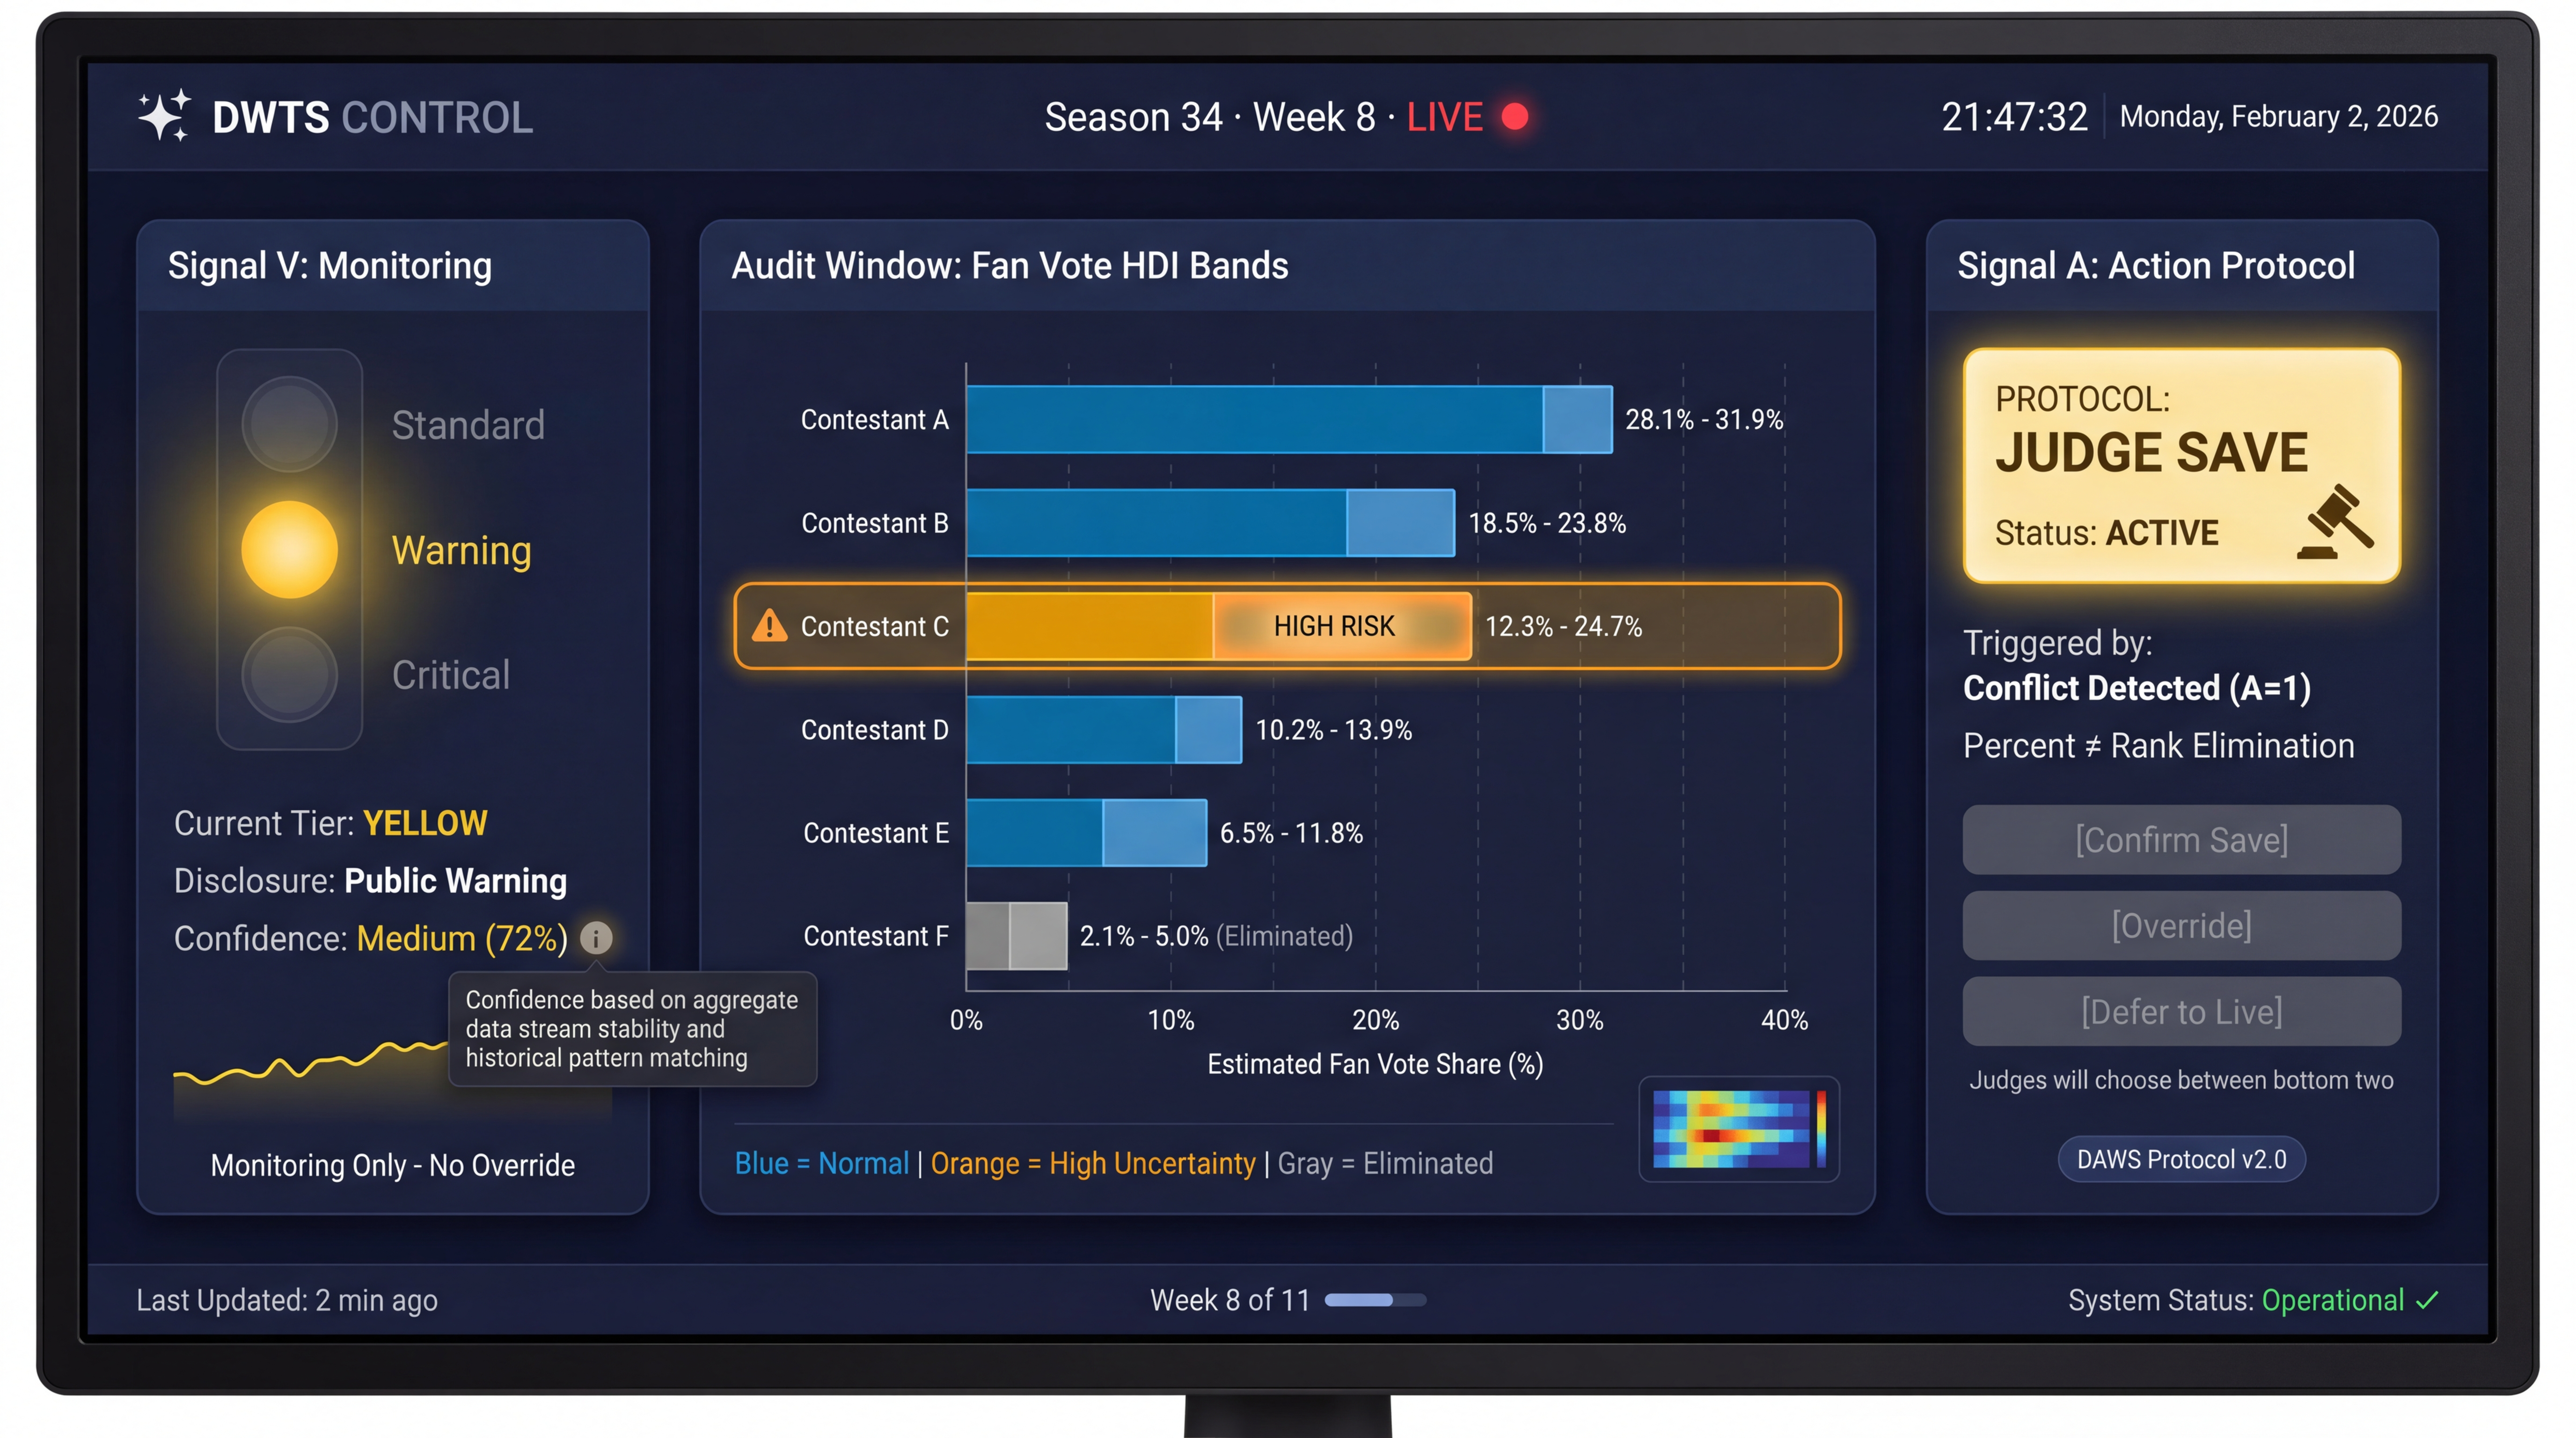
\includegraphics[width=0.98\linewidth]{figures/aigenerate/DAWS.jpg}
\caption{Producer-facing DAWS control dashboard mockup: Signal V monitoring tiers, fan-vote HDI audit window, and the conflict-triggered judge-save protocol (Signal A) in a broadcast-ready decision panel.}
\label{fig:daws-dashboard}
\end{figure}

% 机制对比雷达图
\noindent\begin{minipage}[t]{0.49\linewidth}
\centering
\includegraphics[width=\linewidth]{figures/fig_mechanism_radar.pdf}
\captionof{figure}{Mechanism trade-offs (all weeks; metrics aggregated across weeks).}
\end{minipage}\hfill
\begin{minipage}[t]{0.49\linewidth}
\centering
\includegraphics[width=\linewidth]{figures/fig_mechanism_radar_conflict.pdf}
\captionof{figure}{Mechanism trade-offs (conflict weeks only; when Percent/Rank disagree).}
\end{minipage}

\clearpage
\addcontentsline{toc}{section}{References}
{\footnotesize
\bibliographystyle{unsrt}
\bibliography{ref}
}

\clearpage
\section*{Report on Use of AI Tools}
\addcontentsline{toc}{section}{Report on Use of AI Tools}
\noindent\textbf{Disclosure statement.} We disclose all AI tool usage below, following the COMAP AI policy. AI tools were used only as productivity aids; all modeling choices, equations, code logic, and conclusions were made and approved by the team. No external data beyond the contest dataset were introduced by AI tools.

\noindent\textbf{Representative usage log (abridged).} The entries below summarize prompts and outputs used during development. Outputs were reviewed, edited, and verified by the team before inclusion.
\begin{enumerate}[leftmargin=2em, itemsep=0.9em]
\item \textbf{OpenAI} -- GPT-5.2 Thinking in ChatGPT (model release Dec 11, 2025; ChatGPT model label: ChatGPT-5.2 Thinking; API model: gpt-5.2; accessed Feb 2026).\\
\textbf{Query 1:} Propose a clean module layout for the pipeline (data loading, constraint checks, sampling, and reporting).\\
\textbf{Output:} A modular outline with function boundaries, suggested inputs/outputs, and a call graph; we implemented and adjusted the structure in our codebase.\\
\textbf{Query 2:} Provide a concise Python implementation of a strict feasibility check for elimination constraints on a simplex.\\
\textbf{Output:} A function like the excerpt below (taken from our pipeline after manual edits and testing):
\begin{verbatim}
def strict_feasible_check(
    v: np.ndarray,
    elim_idx: List[int],
    eps_sum: float = EPS_SUM,
    eps_ord: float = EPS_ORD,
) -> Tuple[bool, float, float]:
    """Strict feasible check: simplex + elimination (ties allowed)."""
    simplex_resid = float(abs(float(np.sum(v)) - 1.0))
    if len(elim_idx) == 0:
        elim_resid = 0.0
        ok = bool(simplex_resid <= eps_sum and np.all(v >= -eps_ord))
        return ok, simplex_resid, elim_resid
    n = len(v)
    elim_mask = np.zeros(n, dtype=bool)
    elim_mask[elim_idx] = True
    if np.all(elim_mask) or np.all(~elim_mask):
        elim_resid = float("nan")
        return False, simplex_resid, elim_resid
    max_e = float(np.max(v[elim_mask]))
    min_s = float(np.min(v[~elim_mask]))
    elim_resid = max_e - min_s
    ok = bool(simplex_resid <= eps_sum and np.all(v >= -eps_ord) and elim_resid <= eps_ord)
    return ok, simplex_resid, elim_resid
\end{verbatim}
\textbf{Query 3:} Suggest fixes for shape/index errors when vectorizing the sampling loop.\\
\textbf{Output:} A diagnostic checklist (array shapes, broadcasting rules, and masks) plus a vectorized rewrite; we applied and verified these changes locally.\\
\textbf{Query 4:} Draft a short LaTeX description of the feasibility audit and what the residual means.\\
\textbf{Output:} A paragraph describing simplex residuals and elimination residuals, later edited for clarity and aligned to our notation.\\
\textbf{Query 5:} Provide a brief pseudo-code outline for the sampling pipeline (proposal, filter, summarize).\\
\textbf{Output:} A high-level algorithm outline; we implemented the final version in Python and validated outputs against our metrics.

\item \textbf{Anthropic} -- Claude Opus 4.5 (announcement Nov 24, 2025; API model: claude-opus-4-5; accessed Feb 2026).\\
\textbf{Query 1:} Identify potential edge cases in weekly elimination logic (ties, multiple eliminations, and missing scores).\\
\textbf{Output:} A checklist of cases and suggested guards (tie handling, empty-week checks, and boundary conditions) that we incorporated into validation steps.\\
\textbf{Query 2:} Propose a sensitivity-analysis plan for the sampling scale and judge-fan weight.\\
\textbf{Output:} A stepwise plan (vary seed, vary proposals, vary weight, compare stability and flip rates) used to frame our robustness tests.\\
\textbf{Query 3:} Provide a draft explanation of the DAWS rule in plain language for a general audience.\\
\textbf{Output:} A concise paragraph explaining trigger weeks and judge save logic; we rewrote it to match our final terminology.\\
\textbf{Query 4:} Review the distinction between percent aggregation and rank aggregation for possible ambiguity.\\
\textbf{Output:} A short clarification emphasizing how rank compresses information and can change elimination order; we used this to refine our wording.

\item \textbf{Google} -- Gemini 3 Pro Preview (model ID: gemini-3-pro-preview; preview; accessed Feb 2026).\\
\textbf{Query 1:} Suggest figure types that best communicate uncertainty and rule comparisons.\\
\textbf{Output:} Recommendations for HDI bands, mechanism radar charts, and stability comparison bars; we selected and implemented a subset.\\
\textbf{Query 2:} Rewrite a technical paragraph to reduce ambiguity without changing meaning.\\
\textbf{Output:} A revised paragraph with clearer subject references and shorter sentences; the team edited the final wording.\\
\textbf{Query 3:} Provide a short summary of how to interpret posterior fan-share intervals.\\
\textbf{Output:} A 3-4 sentence explanation used as a draft and then tailored to our notation and results.\\
\textbf{Query 4:} Suggest a succinct figure caption for the mechanism trade-off radar plot.\\
\textbf{Output:} A one-sentence caption highlighting agency, integrity, and stability; we adjusted it to match our final figure labels.

\item \textbf{Google} -- Gemini 3 Pro Image Preview (aka Nano Banana Pro; model ID: gemini-3-pro-image-preview; preview; accessed Feb 2026).\\
\textbf{Query 1:} Image recognition on our figures to identify visual elements (axes, labels, legends, and key regions) for captioning and consistency checks.\\
\textbf{Output:} Detected labels and element descriptions; results were cross-checked against the original figures before inclusion.\\
\textbf{Query 2:} Detect low-contrast text or overlapping annotations in the exported figures.\\
\textbf{Output:} A list of candidate overlaps and low-contrast regions; we adjusted label placement and colors accordingly.\\
\textbf{Query 3:} Confirm axis directions and label ordering on heatmap-style figures.\\
\textbf{Output:} A checklist of axis labels and tick order; we confirmed consistency with the plotted data.
\end{enumerate}

\noindent\textbf{Verification and responsibility.}
\begin{itemize}[leftmargin=2em]
\item We reviewed all AI-assisted outputs for accuracy, consistency, and relevance, and corrected any issues found.
\item We verified that AI outputs did not introduce external data or unsupported claims.
\item We checked all citations and references for correctness and completeness.
\item The team assumes full responsibility for the final report, code, and conclusions.
\end{itemize}

\end{document}
